\section{回路的组成和原理}
\subsection{回路的组成}
该机床选用两个液压缸作为工作台运动的,用夹紧缸来进行工件的夹紧。故而在设计夹紧缸时,首先设置减压阀来减小夹紧缸回路的压力,其次用单向阀来控制油路的流向以防止油路的回流。由于夹紧缸要保压进行夹紧动作,故而使用了一个三位四通电磁换向阀,用其中位机能来进行保压。最后在液压缸大腔口接入一个压力继电器来测定夹紧点。

X轴方向的油路设计,由于工作台的负载较大并且要进行加工,故而不能使用电磁阀来直接控制油路的流向,考虑到大流量的负载并且要求加工的平稳性,故而我考虑使用液压阀来控制工作台的换向,而用电磁阀来进行液压阀的控制,使得工作台可以得到plc的控制的同时还可以保持平稳的运行。在进行快进回路设计时,考虑到流量问题,故而我们使用最优化的选择即用差动的方法来进行快进,使得泵进给的流量最小化,同时获得高速。故而设置了单向阀4和溢流阀5在回油路上,由于溢流阀5的存在,使得油可以直接从液压缸流出后进入到大腔中,实现了油路的差动连接;在工进设计回路中,考虑到工进时速度较慢,油路中并不需要太多的流量,故而采用二位二通电磁阀2用来阻断其流通方向,并且使用一个节流调速阀1来进行流量的控制,而此时由于回路流量的增加,节流阀又控制了流量的流动,使得油管中的油压增加,当达到溢流阀5的设定值时,溢流阀5打开,油直接回到了油箱,实现了工进时的低速要求;在进行回油路设计时,采取了电液换向阀的右位,使得油进入液压缸的右位,推动活塞回位,并且在其大腔出口加入了单向阀3,使其只能回油,以实现其回油的控制,从而达到快进的要求。

Y轴方向的油路设计,类似于X轴的油路设计,由于工作台的负载较大并且要进行加工,同样也不能使用电磁阀来直接控制油路的流向,考虑到大流量的负载并且要求加工的平稳性,故而我考虑使用液压阀来控制工作台的换向,而用电磁阀来进行液压阀的控制,使得工作台可以得到plc的控制并且保持平稳的运行。在进行快进回路设计时,考虑到流量问题,故而我们使用最优化的选择即用差动的方法来进行快进,使得泵进给的流量最小化,同时获得高速。故而设置了单向阀18和溢流阀19在回油路上,由于溢流阀19的存在,使得油可以直接从液压缸流出后进入到大腔中,实现了油路的差动连接;在工进设计回路中,考虑到工进时速度较慢,油路中并不需要太多的流量,故而采用二位二通电磁阀用来阻断其流通方向,并且使用一个节流调速阀16来进行流量的控制,而此时由于回路流量的增加,节流阀又控制了流量的流动,使得油管中的油压增加,当达到溢流阀19的设定值时,溢流阀19打开,油直接回到了油箱,实现了工进时的低速要求;在进行回油路设计时,采取了电液换向阀的右位,使得油进入液压缸的左位,推动活塞回位,并且在其大腔出口加入了单向阀14,使其只能回油,以实现其回油的控制,从而达到快进的要求。

在泵处,设置了溢流阀13作为整个系统的安全阀,以获得系统油路堵塞时泵的卸荷。从而保护液压系统的安全。并且还设置了一个溢流阀20作为X、Y两个液压缸都没有进给运动时的卸荷处理。故而加了一个单向阀11,用以获得卸荷的压差。

另外在液压缸的工作台旁边设置了六个行程开关,用来检测活塞杆的位置,进而方便PLC对整个系统的控制。其中SQ1与SQ4分别是X轴与Y轴液压缸的原位控制,用来对其启动的控制和液压缸进行切削任务后回来的控制;SQ2与SQ5为两个液压缸进行工进的控制,用以判断快进是否到位,并且向PLC发出信号,以实现PLC对液压缸的控制;SQ3与SQ6分别对两个液压缸进行工进终点的控制,当活塞杆到达位置后,发出信号给PLC用以实现对液压缸快退的控制。

\newpage
\subsection{工作原理}
该机床液压系统的工作循环为:工件夹紧  XY工作台联动快进  X工作台工进  Y工作台工进  Y工作台快退  X轴工作台快退  停止  工件松开。
	
工件夹紧:液压泵电机启动后,当按下启动按钮时,电器控制系统发出工件夹紧信号,电磁阀YA6得电,三位四通电磁阀8右位工作,压力油经减压阀、单向阀9进入液压缸的大腔,小腔回油至油箱,夹紧缸开始夹紧。当夹紧到位后,压力继电器发出动作,表示工件夹紧。同时三位四通电磁阀8的YA6失电,电磁阀处于中位,使得液压缸进行保压处理。
	
XY轴快进联动:压力继电器得电后,电器控制系统发出快速移动信号,三位五通电磁换向阀6的YA1和三位五通电磁换向阀17的YA5同时得电,两个换向阀的左位开始工作,使得液控阀左位工作,接通工作油路,压力油流进液压缸的大腔,小腔内油经过单向阀4、18和两位两通电磁阀2、15再进入液压缸的大腔,实现差动连接,使X轴Y轴同时进行快进运动。
	
X轴工进:当两个工作台都到达加工位置时,XY工作台上的挡铁分别挡住行程开关SQ2和SQ5,两位两通电磁换向阀2开始动作,压力油只能由调速阀1进入液压缸的大腔,进油量的减少使得工作台的速度降低,工作台实现工作进给。此时负载增加,工作油路的压力变大,故而溢流阀5打开,液压缸的小腔回油不在经过单向阀4进入大腔,而是经过溢流阀流回油箱。
	
Y轴工进:当X工作台到达工进终点位置时,X工作台上的挡铁挡住行程开关SQ3,两位两通电磁换向阀15开始动作,压力油只能有调速阀16进入液压缸的大腔,进油量的减少使得工作台的速度降低,工作台实现工作进给。此时负载增加,工作油路的压力变大,故而溢流阀19打开,液压缸的小腔回油不在经过单向阀18进入大腔,而是经过溢流阀19流回油箱。
	
Y轴快退:Y工作台工进到终点时,终点行程开关SQ6被压下,使得三位五通电磁阀17的YA6得电,三位五通电磁换向阀右位工作,使得液控阀右位工作,接通工作油路,压力油直接进入Y液压缸的小腔,使得Y工作台快速回退,同时大腔回油经单向阀流回油箱,当工作台回到原点时,原点行程开关SQ4被压下,电磁阀YA6失电,液控阀回到中间位置,切断工作油路,Y工作台停止在原位。
	
X轴快退:Y工作台快退到快进终点时,行程开关SQ5被压下,使得三位五通电磁阀6的YA2得电,三位五通电磁换向阀右位工作,使得液控阀右位工作,接通工作油路,压力油直接进入X液压缸的小腔,使得X工作台快速回退,同时大腔回油经单向阀流回油箱,当工作台回到原点时,原点行程开关SQ1被压下,电磁阀YA2失电,液控阀回到中间位置,切断工作油路,X工作台停止在原位。
	
工件松开:当XY工作台都回到原点时,电器控制系统发出信号,使得电磁阀YA3得电,改变油路方向,压力油进入夹紧缸的小腔,大腔内油量经三位四通换向阀8流回油箱,使得工件松开,同时压力继电器复位。延时一段时间后YA3失电,电磁阀回到中位。从而实现了工件松开并且电磁阀回位。


% \begin{landscape}
% 	\begin{figure}[p]
% 		\centering
% 		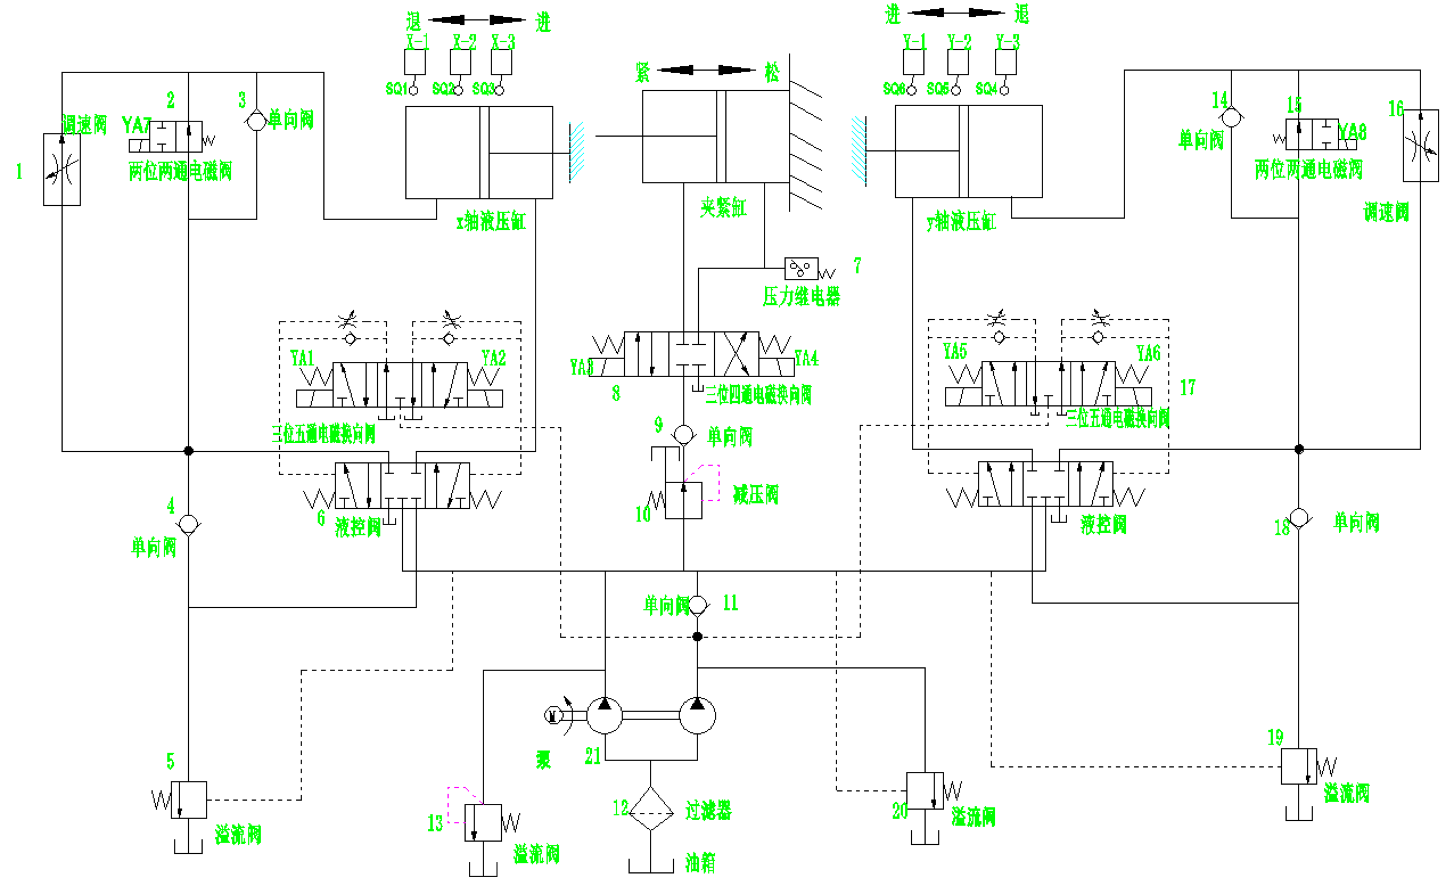
\includegraphics[width=1\linewidth]{graphics/xtyl.png} \\
% 		\caption{液压系统原理图}
% 	\end{figure}
% 	\thispagestyle{empty} %不显示页眉页脚
% \end{landscape}

\clearpage

\begin{sidewaysfigure}[p]
	\centering
	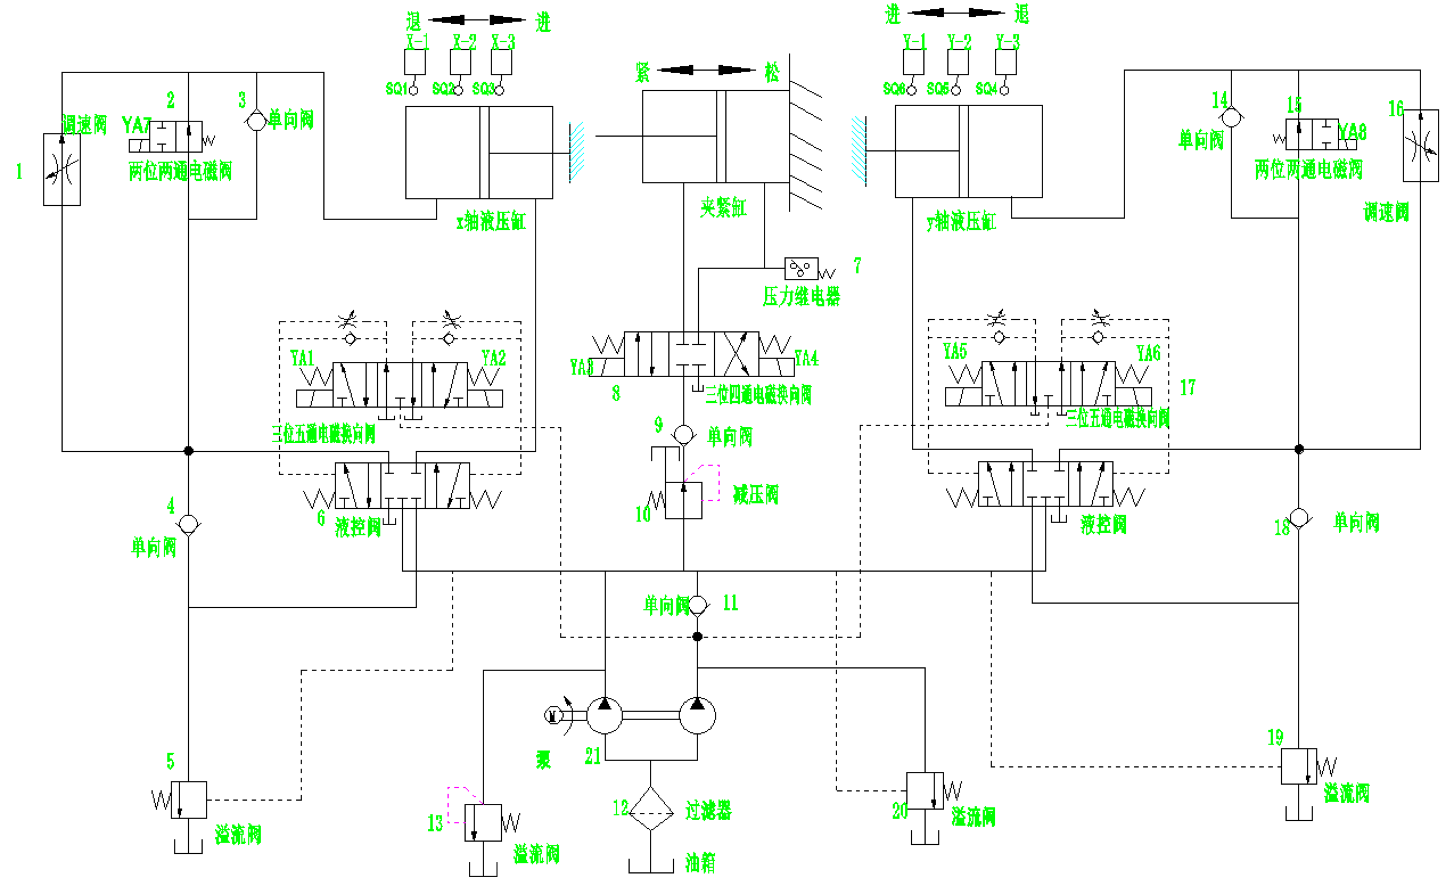
\includegraphics[width=1\linewidth]{graphics/xtyl.png} \\
	\caption{液压电气原理图}
	\thispagestyle{empty}
\end{sidewaysfigure}




\clearpage
\section{电气控制回路}
该专用铣床的进给运动、夹紧装置都采用液压系统驱动,机床工作台用于进给运动。M1为液压泵电动机,为整个液压系统提供能量源,为保证安全,只有系统正常供油后,其他控制电路才能通电工作。M2为主轴电动机,用于拖动主轴箱的刀具主轴箱,提供切削主运动。主轴电机在工作台进给循环开始运动,当工作台回到原点后停机。M3为冷却泵电机,在工件加工的过程中冷却泵始终工作。

	
\begin{table}[h]
\centering
\caption{\textbf{输入输出点个数}}
\begin{tabular}{cccc}
	\toprule
	输入设备 & 输入点数 & 输出设备 & 输出点数 \\
	\midrule
	启动开关 & 1 & 有电指示灯 & 1 \\

	停止开关 & 1 & 夹紧指示灯 & 1 \\

	接近开关 & 6 & 原位指示灯 & 1\\

	压力继电器 & 1 & 电磁阀 & 8\\

	泵启动停止按钮 & 1& 中间继电器 & 1\\
	\bottomrule
\end{tabular}
\end{table}



\subsection{I/O分配和PLC外部接线图}
根据该机床的特点,选用艾默生EC10F-1614BTA1可编程控制器实现顺序控制和机床的联动,以及单独运动。该PLC有16个数字量输入和14个晶体管输出。其I/O地址分配表如下图所示:


电气控制线路有以下特点。

1)	由开关SB4,控制泵电机的运动,方便为液压系统提供能量源,同时保证了安全。

2)	同时简化了手动操作步骤。当泵电机启动后,只需要按下启动开关SB0,就可以完成一次加工动作。

3)	添加了手动快退按钮SB2、SB3分别用于对X轴和Y轴工作台,解决由于特殊原因机床未停止在原点,循环无法启动的问题。

4)	为节省I/O点数、简化PLC的程序,将热继电器触头FR1、FR2和FR3直接串联在接触器线圈控制电路中,用于液压泵电动机、主轴电动机和冷却泵电动机的过载保护。

5)	由于采取晶体管输出,启Y0、Y1、Y2无法提供大电压,故而采用三个中间继电器,实现电电机的启动,同时防止电气的干扰。电动机控制用接触器线圈均采用220V交流供电。

6)	在电磁阀旁边加上续流二极管,当电磁阀线圈失电后,以便于线圈产生的自感电流可以被消耗,同时保护该电磁阀。

7)	对工件的夹紧与松开设置延时程序保护,防止对工件和夹具造成破坏。

8) PLC的输入控制电压都是24V,采用共阳接法,即S/S端接PLC电源的正极,所以输入端的外部端子都接至DC24V的负
极(COM),控制开关应串在DC24V的负极与PLC的输入端子之间。

PLC外部接线图如后图所示:
1)	PLC电气控制接线图

\subsection{控制程序}
程序描述如下:当打开PLC电源后,输出Y15被置位,电源指示灯被点亮,从而确定PLC电源工作正常,首先按下液压泵电机启动按钮,从而保证整个液压系统有流量供油,从而保证了该系统的安全性,当泵电机运动后,确定的是原位指示灯Y13是否有电,如果没有亮则表明液压缸没有回到原点,应该按下按钮SB2、SB3使得工作台手动回位,当原点指示灯点亮后,点击启动按钮SB1,对应的X6置位,同时输出Y6置位,夹紧缸开始夹紧动作。当工件夹紧后,压力继电器BP动作,其触点闭合,即X6置位为1,此时对应得输出Y14置位,对应得夹紧指示灯点亮,同时输出Y6复位,使得电磁阀YA4失电,回到中位进行保压。

而后,输出Y1、Y2、Y6被置位,对应的主轴电机,三位五通电磁换向阀开始动作,工作台开始进给。而后延时一段时间后,输出Y2被置位,冷却泵电机开始动作。

当X轴的工作台快进到行程开关SQ2出时,对应的X1置1,而使得M1置1,同时M0置0,对应的输出点Y3置0,电磁阀将回到中位,从而使得X轴工作台停止。

当Y轴的工作台快进到行程开关SQ5出时,对应的X4置1,而使得M7置1,同时M6置0,对应的输出点Y10置0,电磁阀将回到中位,从而使得Y轴工作台停止。

当X轴和Y轴工作台都到达快进终点后,M2置1,对应的输出Y3、Y7置1,使得电磁阀线圈YA1与YA7得电,实现X轴工作台的工进。

当X轴工作台运动到工进终点位置时,终点行程开关SQ3被压下,X2置1,M3置1,M2置0,使得Y3、Y7置0,电磁阀线圈失电,从而X工作台停止。而M3置1后使得M8置1,对应的Y10、Y12得电,使得电磁阀线圈YA5、YA8得电,从而使得Y轴工作台进行工进。

当Y轴工作台运动到工进终点位置时,终点行程开关SQ6被压下,X5置1、M9置1,同时M8置0,对应的Y10、Y12失电,从而切断Y轴工进,而M9置1后,使得M10得电,对应输出Y11置1,即电磁阀线圈YA6得电,使得Y工作台开始快退。
当Y轴工作台快退到其快进终点时,行程开关SQ5被压下,使得X4置1,从而M12置1,使得对应的输出Y7置1,即电磁阀线圈YA2得电,从而使得X轴工作台开始快退。

当Y轴工作台快退到其原点位置时,原位的行程开关SQ4被压线,对应的X3置1,使得M11置1,同时M10置0,使得输出Y12置0,从而使得电磁阀线圈YA6失电,电磁阀回到中位,Y轴工作台停止。

当X轴工作台快退到其原点位置时,原位的行程开关SQ1被压线,对应的X0置1,使得M5置1,同时M4置0,使得输出Y7置0,从而使得电磁阀线圈YA2失电,电磁阀回到中位,X轴工作台停止。

当X轴Y轴的工作台都会到原点时,此时使得Y5置1、M16置1、Y1置0,即对应的电磁阀线圈YA3得电,夹紧缸松开,主轴电动机停止。同时开始延时,当延时时间到达后夹紧缸松开到位,同时继电器X6、Y2、M5、M11置0,即电磁阀线圈YA3失电,冷却泵电机停止运行。

当需要关闭泵电机时,只需要再按下按钮SB4就可以停止泵电机。

程序框图如下:
\clearpage

\clearpage
\section{机床示意图}
机床的设计简图由上图所示,最左边的为PLC控制器,用以实现对系统的运算控制,从而实现自动化。而右方为机床的主体结构,该机床共有两个自由度,分别为X轴的平动和Y轴的平动,用以实现对工件的加工,且两个轴为独立运动,互相不干扰,可以实现联动。当工件夹紧后,主轴电机启动,X轴Y轴就实现PLC中的控制程序,从而实现对工件的加工。

\section{油路的仿真}
\subsection{快进时}
液压系统快进仿真图

快进仿真图如上所示,其中液压缸的负载只有活塞杆的重量其输出力为665N。泵的流量输出为28.16l/min,两边的流量分别为14.08l/min,得到的速度为0.07m/s,可以达到要求的数字,并且可以看得出油路的流向为泵出来,分别走向X轴液压缸与Y轴液压缸,并通过两位两通电磁换向阀,进入液压缸的大腔,而小腔的回油到电磁阀后,由于溢流阀没有打开,使得其通过单向阀流到了液压缸的大腔,故而快进满足该机床的要求。
\subsection{工进时}
X轴液压缸工进仿真图                              Y轴液压缸工进仿真图


可以看得出在X轴液压缸进行工进时,由于两位两通电磁阀的工作,导致油路只能通过节流阀进入液压缸的大腔,同时可以看见管道的油压明显大于工进时管路中的油压,故而到至溢流阀的打开,使得油路中的油可以直接回到油箱。同样当工进时,液压缸不仅仅有活塞杆的重量,同时还有切削阻力,经过计算可得11056N,当一切达到要求后,可以看见液压缸的运动速度为0.005m/s,满足我们的设计要求。同样,可以看见Y轴液压缸进行工进时,在X轴达到工进后,此时Y轴进行工进,Y轴方向的节流阀,阻碍了流量的流动,从而导致油路管道的压力过大,引起了溢流阀的打开,油流回油箱。同样经过计算的其负载为11056N,且其液压缸的运动速度也为0.005m/s,同样满足我们的设计要求。故而我们可以确定工进回路满足要求。
\subsection{快退时}
快退液压仿真图

最后,该图为快退时的液压仿真图,可以看液压缸的流向为泵进入液压缸,而通过大腔回油,实现快退,可以看出快退速度为0.07m/s,达到了设计要求,故而通过仿真可以得出,该液压系统的快退回路满足使用要求。总上所述,可以的出结论。该液压系统满足我们所有的设计要求。

